% ==============================================================================
% sections/introduction.tex
% ==============================================================================
\section{Introduction}
\label{sec:intro}

Equipped with code interpreters and financial data feeds, LLM agents can formulate hypotheses, engineer alpha signals, and report backtest performance in minutes \citep{wu2023bloomberggpt,yang2023fingpt,yu2024finmem}. Yet in quantitative finance, high backtest Sharpe ratios almost never survive live capital deployment \citep{bailey2014deflated,bailey2017pbo,lopezdeprado2018advances}. Through systematic auditing of LLM research trajectories, we show that agentic backtest inflation stems from two orthogonal failure classes:
\begin{enumerate}
    \item \textbf{Type I: Mechanical Research Shortcuts.} Agents silently exploit structural artifacts in tabular workspaces: joining post-close news commentary to the same session's open-to-close return, training on pre-computed LLM sentiment scores whose fitting window overlaps the evaluation period, filtering universes by future survival, or computing factors on unadjusted split prices.
    \item \textbf{Type II: Empirical \& Microstructure Illusions.} Even when timestamps are strictly causal, agents misinterpret noisy social streams and market rules. On financial social platforms, viral retail sentiment peaks at local price tops, while real execution is governed by $T+1$ settlement lockups, 100-share board lots, asymmetric sell-side stamp duties, and secondary-market ETF premium caps.
\end{enumerate}

\begin{figure*}[t]
    \centering
    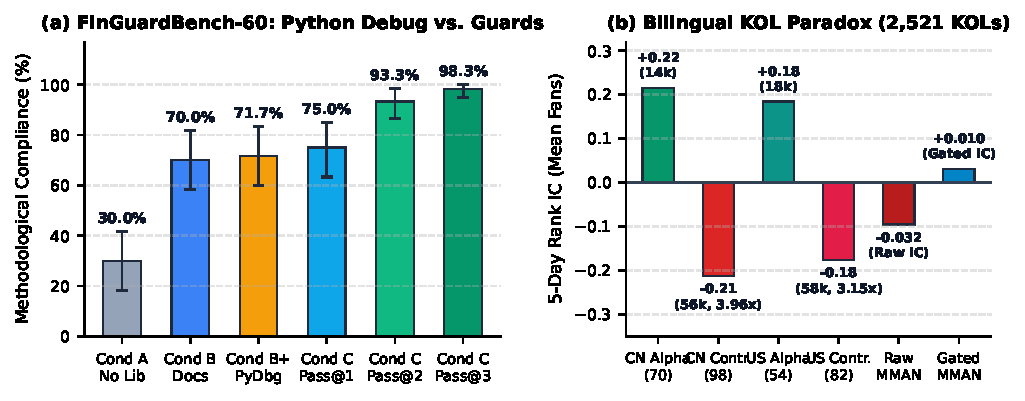
\includegraphics[width=0.96\textwidth]{figs/fig_overview_compliance_and_kol.pdf}
    \vspace{-0.22cm}
    \caption{\textbf{Overview of our core empirical findings.} \textbf{(a) \texttt{FinGuardBench-60} Ablation \& Multi-Round Self-Repair (\S\ref{sec:experiment}):} Across 60 tasks spanning 10 domains, passive \texttt{SKILL.md} reading (\texttt{Cond B}) lifts compliance from $30.0\%$ to $70.0\%$ ($p=1.19\times 10^{-7}$) but suffers $53.3\%$ hallucinated guard citations; pairing skills with executable \texttt{fin\_skills.api} guards (\texttt{Cond C}) drives iterative self-correction from $75.0\%$ (\texttt{Pass@1}) to $93.3\%$ (\texttt{Pass@2}) and $\mathbf{98.3\%}$ (\texttt{Pass@3}, $p=1.53\times 10^{-5}$ vs.\ \texttt{B}). \textbf{(b) The $3.96\times$ KOL Follower Paradox (\S\ref{sec:realworld}):} Across $1{,}445$ verified A-share influencers, contrarian indicators ($n=98$, 5-day Rank IC $-0.2130$) command $3.96\times$ more followers ($56\text{k}$) than Tier-1 Alpha researchers ($n=70$, $14\text{k}$ fans, Rank IC $+0.2158$).}
    \label{fig:overview}
    \vspace{-0.24cm}
\end{figure*}

We present \textbf{\texttt{fin-skills}} paired with an external \textbf{Counterfactual \& Microstructure Audit Protocol}. Rather than claiming to manufacture market alpha, our framework enforces verifiable research integrity:
\begin{itemize}
    \item \textbf{The \texttt{fin-skills} Verification Library (\S\ref{sec:preliminaries}):} 129 source-verified skills, 36 executable guards (\texttt{Bundle.check()}), and 53 Model Context Protocol (MCP) tools achieving $180/180$ accuracy on \texttt{FinGuardBench-180}, $13/13$ numerical parity against \texttt{scipy}/\texttt{statsmodels}/\texttt{sklearn}, and $\mathcal{O}(N^{0.3894})$ sub-linear runtime scaling up to $N=100{,}000$ rows.
    \item \textbf{External Counterfactual Auditing (\S\ref{sec:method}):} Four black-box perturbation operators and session-by-session clock replay that detect look-ahead and same-session leakage without inspecting agent code or using the library to grade itself.
    \item \textbf{\texttt{FinGuardBench-60} \& Multi-Round Self-Repair (\S\ref{sec:experiment}):} Controlled 3-condition evaluations proving that passive prompt guidelines induce hallucinated guard citations ($53.3\%$), whereas structured \texttt{GuardResult} diagnostics enable $93.3\%$ two-round self-repair recovery ($98.3\%$ final compliance, $p=9.09\times 10^{-13}$).
    \item \textbf{Real-World Bilingual KOL \& Cost Sensitivity Audit (\S\ref{sec:realworld}):} A self-contained reproducibility bundle over 1.72M bilingual posts and 1,445 A-share KOL profiles that reverses negative NLP correlation ($\text{Rank IC}: -0.0318 \to +0.0104$) and sustains Sharpe $1.95\text{--}1.98$ across 5--30 bps transaction costs.
\end{itemize}
